\subsection{Вычислительные эксперименты}
    Возьмём такие функции для построения модели:
    \[
        \begin{split}
            & \varepsilon (x_1) = -x_1 + 10, \\
            & K_{12} (x_1) = x_1 - 5, ~ K_{13} (x_1) = x_1 - 3, ~ K_{23} (x_2) = x_2 - 4, \\
            & V_{12} (x_1) = 2 x_1, ~ V_{13} (x_1) = 3 x_1, ~ V_{23} (x_2) = x_2.
        \end{split}
    \]

    \subsubsection{При вымершей первой популяции}

    \begin{figure}[H]
        \centering
        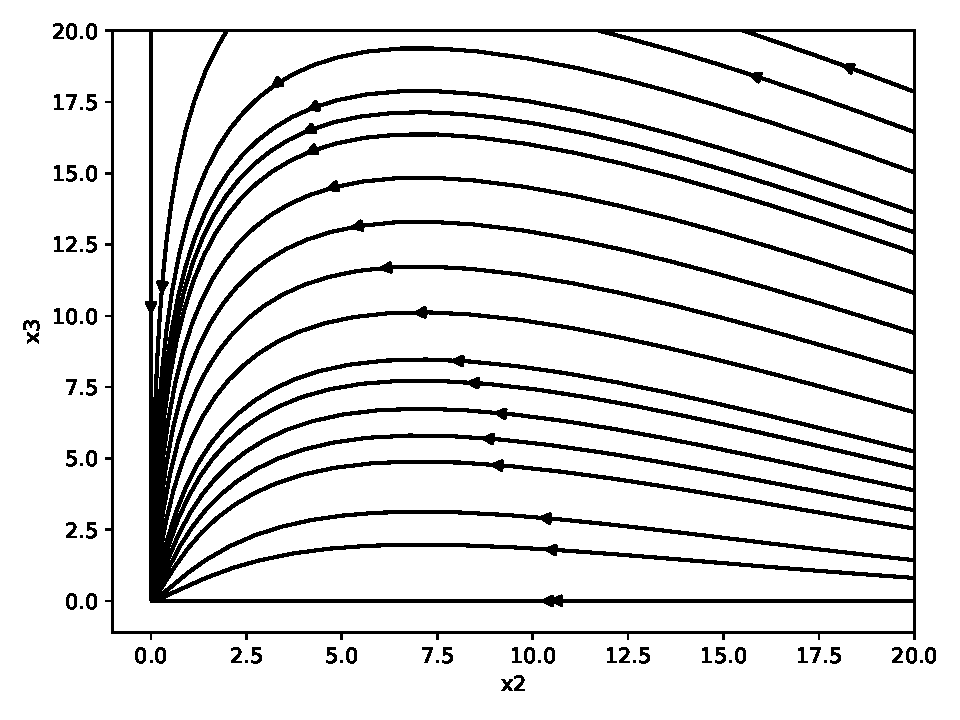
\includegraphics[width=8cm]{pictures/kx1_0vector.pdf}
    \end{figure}


    \subsubsection{При вымершей второй популяции}

    \begin{figure}[H]
        \centering
        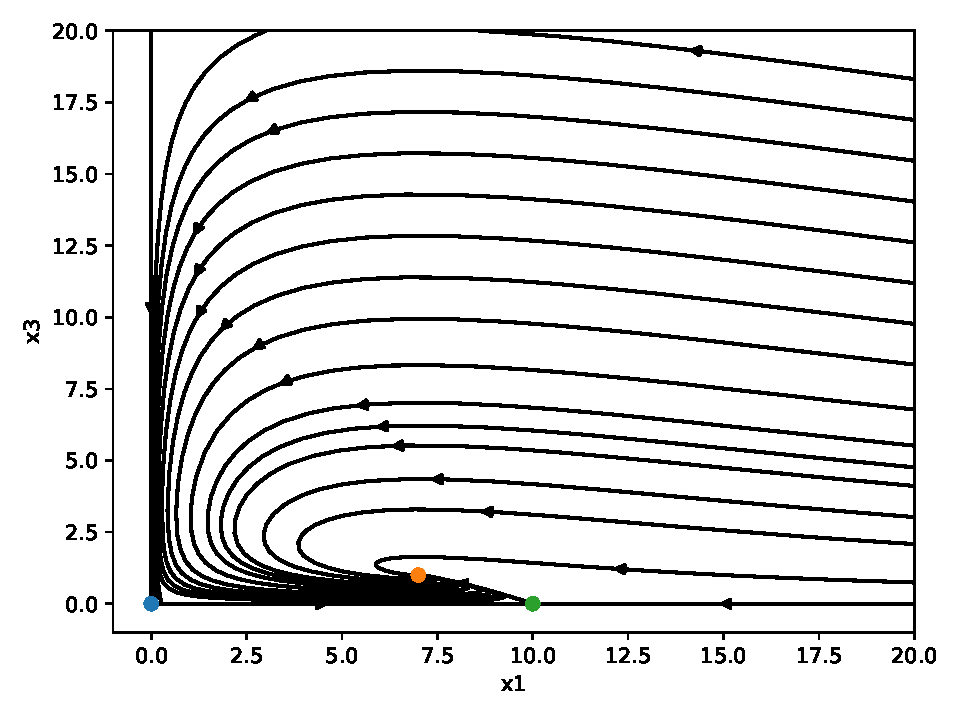
\includegraphics[width=8cm]{pictures/kx2_0vector.pdf}
    \end{figure}


    \subsubsection{При вымершей третьей популяции}

    \begin{figure}[H]
        \centering
        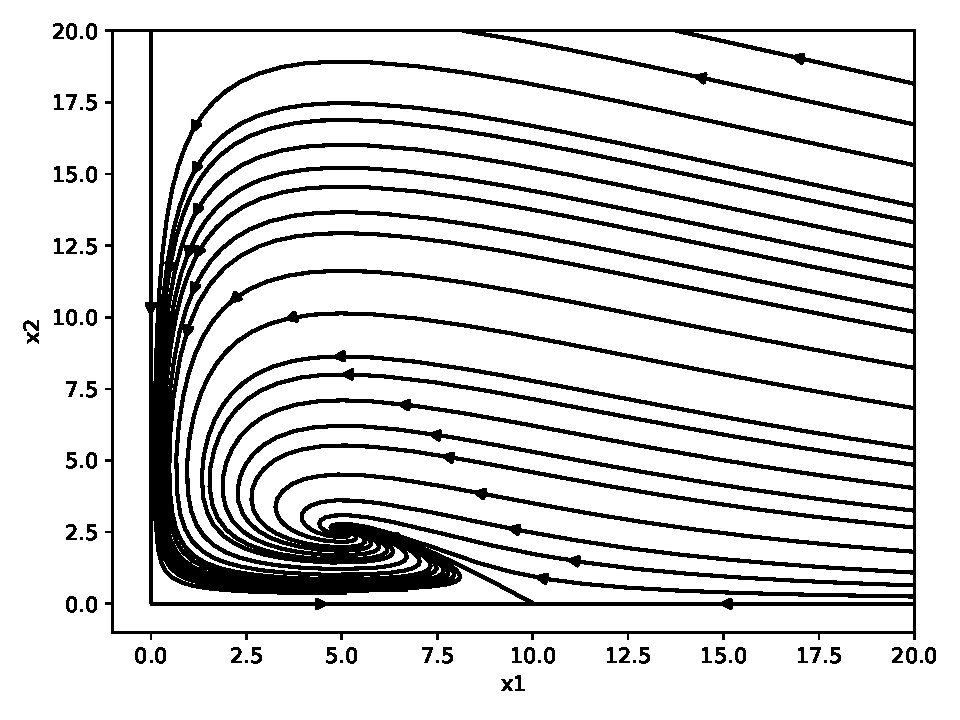
\includegraphics[width=8cm]{pictures/kx3_0vector.pdf}
    \end{figure}

    \subsubsection{Несколько изначально не вымерших популяций}
    \begin{figure}[H]
        \centering
        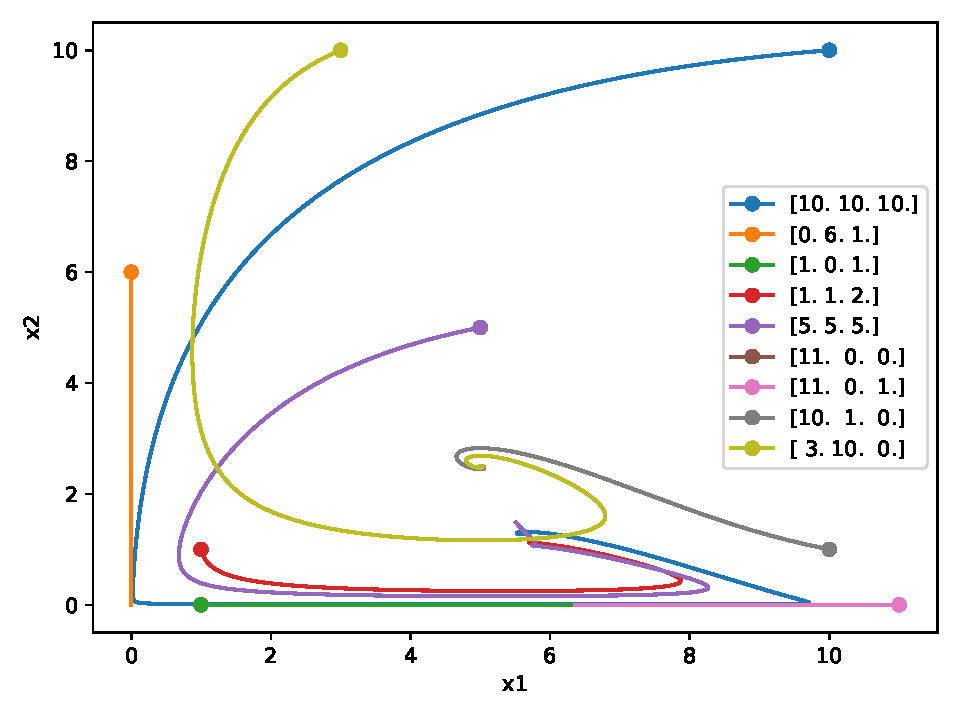
\includegraphics[width=8cm]{pictures/kx_12phase.pdf}
        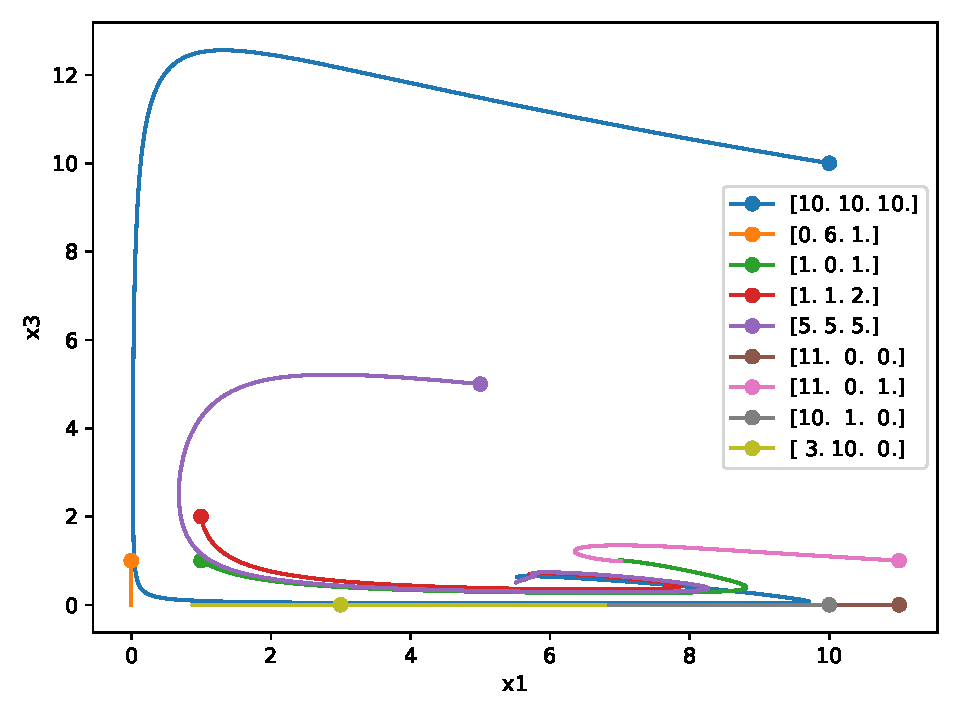
\includegraphics[width=8cm]{pictures/kx_13phase.pdf}
        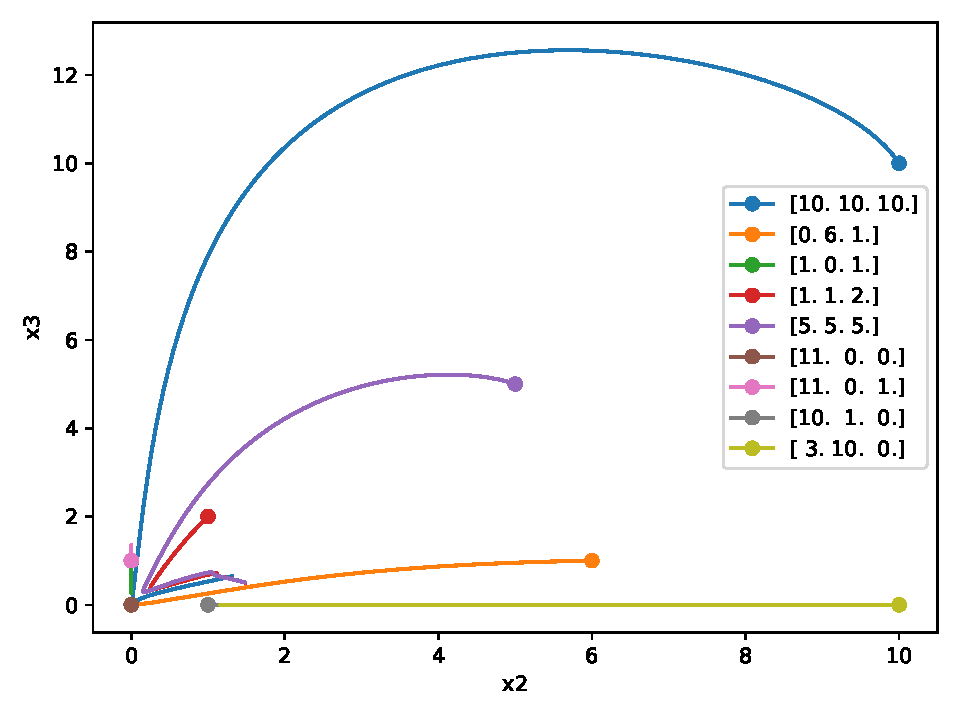
\includegraphics[width=8cm]{pictures/kx_23phase.pdf}
        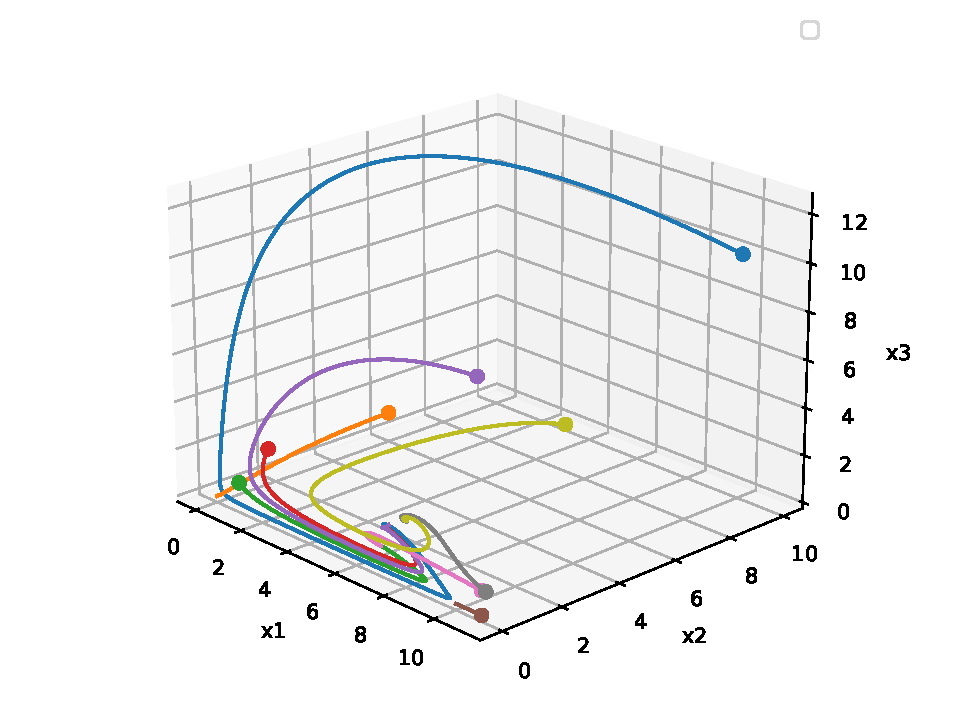
\includegraphics[width=8cm]{pictures/kx_phase3.pdf}
        \caption{На отрезке времени \( [0, 3] \).}
    \end{figure}